\documentclass[a4paper]{proc}

\usepackage[utf8]{inputenc}
\usepackage[T1]{fontenc}
\usepackage[english]{babel}
\usepackage{graphicx}
\usepackage{url}
\usepackage{indentfirst}

\author{Paul MABILEAU\\\texttt{paul.mabileau@telecom-sudparis.eu} \and Franck STAUFFER\\\texttt{franck.stauffer@telecom-sudparis.eu}}
\title{\textbf{Recursive Inter-Network Architecture's Security}}

\begin{document}
\maketitle
\tableofcontents
\newpage
\part*{Introduction}
The Recursive Inter-Network Architecture (RINA) is a network architecture based on Internet Process Communication (IPC) presented as an alternative to TCP/IP\@.
It was designed a while ago without security in mind. 
It has been patched to include security but it creates complexity.\cite{assessing-security}

\part{Comparing RINA against TCP/IP}
\section{Distibuted Application Facility}
The smallest part of RINA is the Distributed Application Process (DAP) which is a process running on a host, if at least two of them communicate it is called a Distributed Application Facility (DAF).
They communicate with objects structured in a Resource Information Base (RIB) that define naming and structure. (figure~\ref{daf})\\
They use a Common Distributed Application Protocol (CDAP) that permit to execute 6 operations on a distant DAP's objects:
\begin{itemize}
\item create
\item delete
\item read
\item start
\item stop
\item write
\end{itemize}
The DAF can be compared to the Application layer on the TCP/IP model. DAPs need underlying `layers' to communicate.\cite{wiki}

\begin{figure}
    \centering
    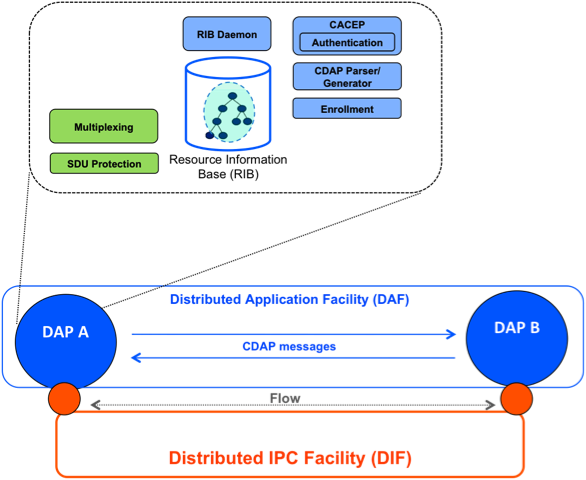
\includegraphics[width=0.9\columnwidth]{DAF.png}\label{daf}\caption{Base of RINA's architecture}
\end{figure}

\section{Distributed IPC Facility}
A Distributed IPC Facility (DIF) is a DAF but instead of containing DAPs, it contains IPC Processes (IPCPs).
It can be compared to a layer in the TCP/IP model but there is not a fixed amount of DIFs, the number can be adapted to the needs of a specific network.

\part{Security provided by RINA's conception}
\section{Authentication}

\par In RINA, authentication is mandatory. This is one of the major, if not the
most important security feature of the architecture, as previous security
analysis often consider attacks plausible only after a successful authentication
\cite{assessing-security, wiki, PINS}.

\par Authentication occurs before a process may communicate on a DIF, either by
creating a new one, or by joining an existing one, and is verified by the
destination application process. When creating a brand new DIF, the initial IPC
process simply has to exist in order to let others join the newly created DIF.
When joining an already existing DIF, the joining process asks permission to the
destination process it wants to communicate with. It achieves this using a
subsequent DIF that both processes have in common and are authenticated in.
The destination process is the one that determines whether the joining one has
sufficient rights through any sort of authentication, described in the DIF's
policy. It may be as strong or weak as desired by the DIF and for the wanted
communication. Then, the destination process gives the joining one a new
node address so it may communicate on the newly joined DIF with.

\par This design feature is quite useful for hardening security considerations
in network communications, as being authenticated \textit{every time} means that
the destination application decides who to talk with and how strict this
decision is using policies, \textit{every time}. It thus builds greater trust
between applications through native access control.

\section{Strict encapsulation}

\par Encapsulation is a very common paradigm for network communications, as it
helps in keeping functionally different parts of the global system separate in
conception as well as in usage. However, the historical TCP/IP model chose to
apply this by function rather than by scope. This means that separation of
concerns is relatively poorly achieved because a certain layer needs to know a
certain amount of information about its subsequent layer(s) in order to properly
work and deliver the expected service. For example, when establishing an HTTP
connection, the client has to:
\begin{enumerate}
    \item Resolve the IP address through the Domain Name System (DNS). One could
        argue that this constitutes a two-level layer leakage, as it crosses TCP
        and IP.
    \item Use the resulting IP address in the transport layer (TCP) in order to
        establish a connection.
    \item Suppose the correct destination port using well-known ports.
\end{enumerate}
This renders the communication not ideal.

\par On the contrary, RINA deals with layers in a stricter way: a process may
only use the functions of a DIF below it is connected to and serve the
application that is above it. It is not supposed to guess or determine
information about inferior or superior DIFs. This is the recursive property of
RINA. Although it may seem simple, it is a fundamental rewind: at any level in
the communications stack a DIF can decide to encrypt or hash its data units if
it does not trust its inferior DIF in order to achieve confidentiality or
integrity. One can thus easily imagine the amount of protection reinforcements
that can be achieved with this, which could be loosely compared to The Onion
Router (TOR) project that offers many public and free network relays so users
may connect to a remote web site only through a circuit of these machines with
additional encryption between each of them. This project exists mainly for
privacy concerns, but it still illustrates the possibilities at hand.


\part{(optional) The threats to RINA}

\nocite{*}
\newpage
\bibliographystyle{unsrt}
\bibliography{report}
\end{document}
